\documentclass[12pt]{article}
%\usepackage[margin=1in]{geometry}

\setlength{\oddsidemargin}{0.25 in}
\setlength{\topmargin}{-0.6 in}
\setlength{\textwidth}{6.5 in}
\setlength{\textheight}{8.5 in}

\setlength{\headsep}{0.75 in}
\setlength{\parindent}{0 in}
\setlength{\parskip}{0.1 in}
\usepackage{xcolor}
\usepackage{graphicx}
\usepackage{subcaption}
\usepackage{mwe}
\usepackage{dirtytalk}
\usepackage{amsmath,amsfonts}

\usepackage{makecell} 
\usepackage{algorithm,algcompatible}
\usepackage{float}
\usepackage[a4paper,bindingoffset=0.2in,%
            left=0.5in,right=0.5in,top=0.5in,bottom=0.5in,%
            footskip=.25in]{geometry}

\newcounter{lecnum}
\renewcommand{\thepage}{\arabic{page}}
\renewcommand{\thesection}{\arabic{section}}
\renewcommand{\theequation}{\arabic{equation}}
\renewcommand{\thefigure}{\arabic{figure}}
\renewcommand{\thetable}{\arabic{table}}
\usepackage{listings}
\usepackage{kotex}
\usepackage{times}

\newcommand{\lecture}[4]{
   %\pagestyle{myheadings}
   %\thispagestyle{plain}
   \newpage
   \setcounter{page}{#3}
   \noindent
   \begin{center}
   \framebox{
        \vbox{\vspace{2mm}
        \hbox to 6.28in { {\bf 2023 Academic English Research report
	       \hfill 2023.11.14.} }
        \vspace{4mm}
        \hbox to 6.28in { {\Large \hfill \textbf{#2} \hfill} }
        \vspace{2mm}
        \hbox to 6.28in { { Name: \textbf{#1} \hfill } }
        \vspace{2mm}}
   }
   \end{center}
}

\renewcommand{\cite}[1]{[#1]}
\def\beginrefs{\begin{list}%
        {[\arabic{equation}]}{\usecounter{equation}
         \setlength{\leftmargin}{2.0truecm}\setlength{\labelsep}{0.4truecm}%
         \setlength{\labelwidth}{1.6truecm}}}
\def\endrefs{\end{list}}
\def\bibentry#1{\item[\hbox{[#1]}]}

\newcommand{\fig}[3]{
			\vspace{#2}
			\begin{center}
			Figure \thelecnum.#1:~#3
			\end{center}}
\newtheorem{theorem}{Theorem}[lecnum]
\newtheorem{lemma}[theorem]{Lemma}
\newtheorem{proposition}[theorem]{Proposition}
\newtheorem{claim}[theorem]{Claim}
\newtheorem{corollary}[theorem]{Corollary}
\newtheorem{definition}[theorem]{Definition}
\newenvironment{proof}{{\bf Proof:}}{\hfill\rule{2mm}{2mm}}

\newcommand\E{\mathbb{E}}

\begin{document}
\lecture{Jinmo Ahn}{The Effect of Caffeine on ADHD }{1}{2017160111}

\section{Background Knowledge}
\subsection{Idea}
\quad There are many stimulants in the world, such as beta-alanine and arginine, but caffeine is by far the most widely used. It's often used when you want to perform explosively, especially during high-intensity workouts or school exams. One of the best features of caffeine is that it's very fast acting, with an average peak in 0.5 to 1 hour. So, why not use this great drug for therapeutic purposes instead of performance? I was intrigued by this question and broke down the topic. I was interested in ADHD, which has become an issue in recent years due to technological advancements, and since the most commercially available ADHD medication, "Methadate Concerta", has numerous side effects, I thought it would be worth studying if caffeine, which is relatively safe, could be used as an alternative. Therefore, I decided to combine caffeine and ADHD under the title "The effect of caffeine on ADHD". 
\subsection{Relevant Study}

\begin{figure}[h]
    \includegraphics[width = 14cm]{kk1.png}
    \centering
    \caption{Caffeine to Frontal lobe}
\end{figure}
\quad There have been numerous studies linking caffeine and ADHD, but the first was published in 2003, "Caffeine and central noradrenaline: effects on mood, cognitive performance, eye movements and cardiovascul". In healthy adult males, the study showed that caffeine had a positive effect on mood compared to placebo, specifically increasing alertness and contentment, and a positive effect on cognitive performance, specifically attention and vigilance. A more recent study that has since become more relevant is J.C.V.'s "Effects on Caffeine consumption on Attention Deficit Hyperactivity Disorder Treatment : A Systematic Review of Animal Studies" from 2022. To summarize the findings of the paper, caffeine improves learning and memory impairments associated with attention deficit, while having no effect on blood pressure and weight. These results are supported at the neuronal/molecular level. However, several propositions (such as activity and impulsivity) caused inconsistencies, suggesting that further research is needed.

\subsection{Study Aims and Expectation}

\quad My research is designed to define the presence of correlation between Caffeine Consumption and ADHD with ADHD-self-recognition. The hypothesis of the research is that Caffeine has good effects on Cognitive ability system 
\\
\\

\section{Own Survey}
\subsection{Demographics}
 \quad We primarily surveyed freshmen taking Academic English classes at Korea University, with an additional survey of a few junior and senior students in the Physics Department at Korea University. Participant's age is 20 to 25, Various other elements are not collected for privacy purposes.

\subsection{Methodology}
\quad We conducted our research online using Google Forms and did not conduct any offline research. For privacy reasons, we did not collect any emails or personal information. And Question is Simply about ADHD test, Caffeine Consumption and ADHD-self-Recognition.

\subsection{Data Collection}
\quad Number of our question is six. and It contains one question about caffeine consumption, four for ADHD test and one for ADHD-self-recognition. Caffeine-consumption question simply means about "how much caffeine does participants consume by any kinds of consumption.". ADHD test is powerfully wired to "Clinical partners" which is world widely credible site. Finally, last question is just asking "How do participants think about them".
\subsection{Data Analysis}
\quad My data analysis contains some different way. Because naive Data has less tendency than I thought. 
\\
First, I will use  quantization method to draw a line between "Applicable property" and "None-applicable property".
\\
Second, The two categorized groups are easier to analyze about tendency, and plot a graph.
\\
Third, Analyze the graph and emphasize my own opinion. Final stage is finding grounds about opinion.
\newpage
\section{Result}

\subsection{Naive data plotting}
\begin{figure}[h]
    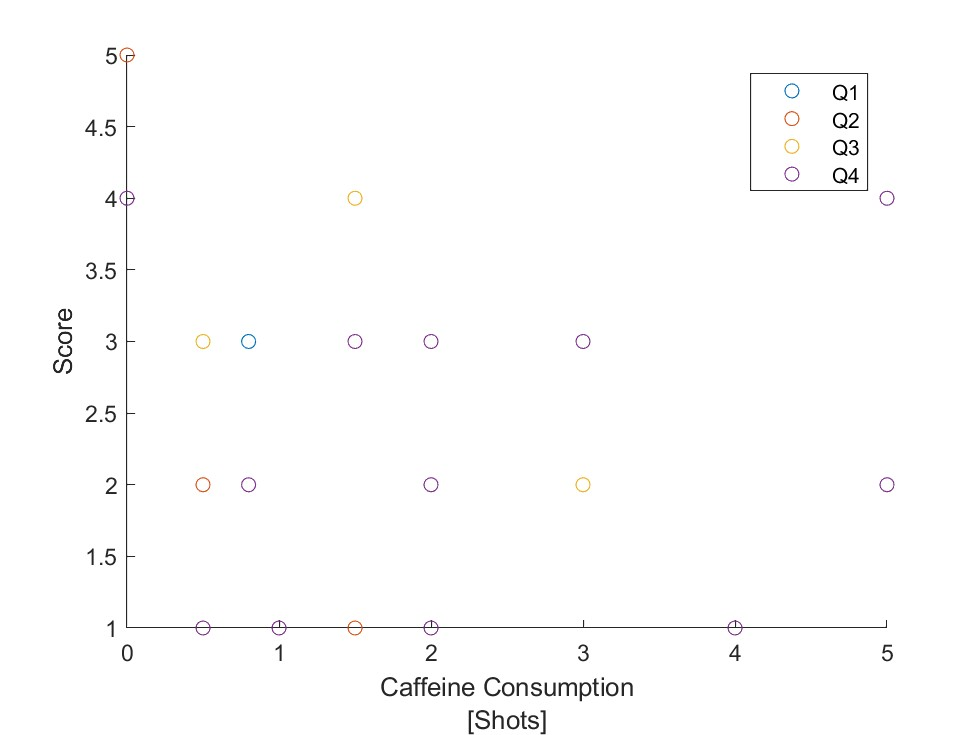
\includegraphics[width = 10cm]{pic1.jpg}
    \centering
    \caption{Caffeine vs ADHD test score}
\end{figure}
\quad Above graph is naively fitting a scatter plot about "caffeine consumption vs ADHD test score". And I cannot fine any tendency between two properties. But I can find that lower caffeine consuming participants has lower score. With that in mind, I will analyze the data. 

\begin{center}
    
\end{center}
\begin{figure}[h]
    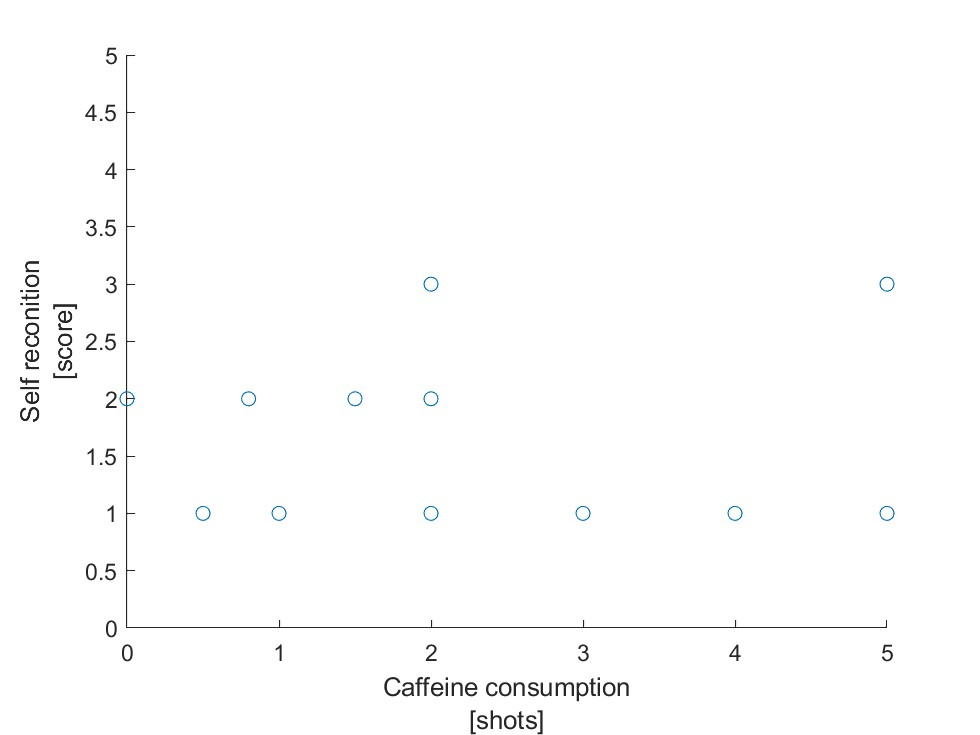
\includegraphics[width = 10cm]{pic2.jpg}
    \centering
    \caption{Caffeine vs ADHD-self-recognition score}
\end{figure}
\quad Above graph is naively fitting a scatter plot about "caffeine consumption vs ADHD-self-recognition score". And I cannot fine any tendency between two properties. Interesting thing is plenty caffeine consumers(over 3) rarely think ADHD themselves. With that in mind, I will analyze the data.

\subsection{Modified data plotting}
\quad I will divide participants into two groups. One is "Caffeine-megadoser (three or more shots per day) " and The other one is "non-megadoser (less than three shots per day)". 
\begin{figure}[h]
    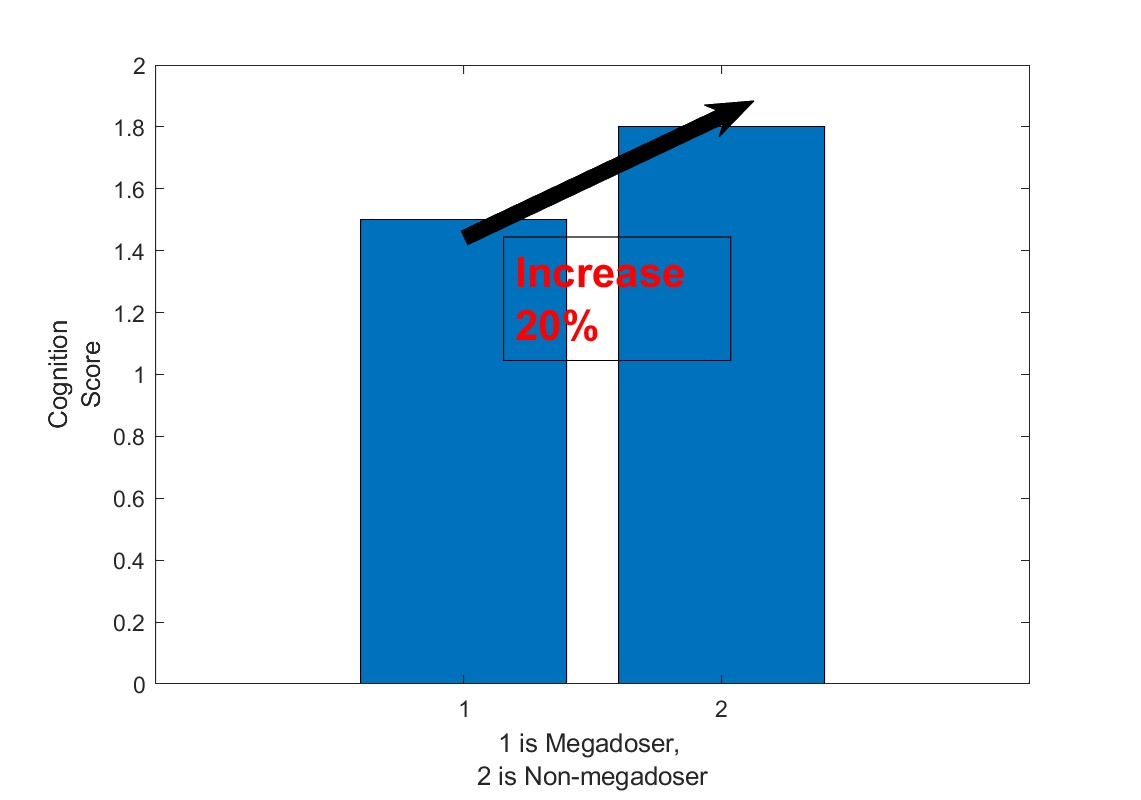
\includegraphics[width = 12cm]{pic3.jpg}
    \centering
    \caption{Megadoser vs Non-megadoser (ADHD-self-recognition score)}
\end{figure}

\quad I found that megadosers were less likely to consider themselves ADHD. they were 1.2x more likely to do so than non-megadosers. This also suggests that a megadose of caffeine makes individuals feel more focused.

\begin{figure}[h]
    \includegraphics[width = 12cm]{pic4.jpg}
    \centering
    \caption{Megadoser vs Non-megadoser (ADHD-test score)}
\end{figure}

\quad I found that megadosers were actually not related with ADHD. they were 1.2x more likely to do so than non-megadosers. This also suggests that a megadose of caffeine makes individuals actually more focused.
\newpage
\section{Conclusion}
\quad In my research, I've found that caffeine can make an individual feel like they're focused, and in fact, they are. What's even more interesting is that the degree to which people feel they have ADHD is proportional to the degree to which they actually do. In other words, what makes you feel focused is what makes you actually focus. In this case, it was simply caffeine, but there are many other stimulants in our life, including beta-alanine, coenzyme Q, and more. If they were to be effective in actual ADHD treatment, they could replace the current popular "metadate concerta".

\section{Limitation and Follow-up research}
\quad I think my major mistake is not checking side effects of megadose. Because, I had no idea my research flow would lead to this. And it is my research's first limitation. Second limitation is too biased sample. My sample is University student who is 20~26 years old. And they are so-called "medicine works like a charm". So, Caffeine may not work as well for the elderly or infants. This is my second limitation. But as you know, It is operating very well to specific sample (university students). So it's both an advantage and a disadvantage.
\\
\quad To overcome this limitations, We have to extend the caffeine to any kinds of stimulants.
and Enlarging the sample size, university students to all ages. 
Finally, we have to check about side effects.

\section{Reference}
1. Smith, A., Brice, C., Nash, J., Rich, N., and Nutt, D. J. (2003, September). Caffeine and Central Noradrenaline: Effects on Mood, Cognitive Performance, Eye Movements and Cardiovascular Function. Journal of Psychopharmacology, 17(3), 283–292. https://doi.org/10.1177/02698811030173010 \\
2. Vázquez, J. C., Martin de la Torre, O., López Palomé, J., and Redolar-Ripoll, D. (2022, February 10). Effects of Caffeine Consumption on Attention Deficit Hyperactivity Disorder (ADHD) Treatment: A Systematic Review of Animal Studies. Nutrients, 14(4), 739. https://doi.org/10.3390/nu14040739\\
3. ADHD Test Online | Clinical Partners. (n.d.). https://www.clinical-partners.co.uk/for-adults/adult-adhd-add/test-for-adhd/test

\newpage
\section{Appendix}
\subsection{Questions}
Q1. On Average, how many caffeinated beverages ( something likes coffee, energy drinks, etc) do you consume per day?
(You can type irrational number but positive only)
\\
\\
Q2.How often do you have trouble wrapping up the final details of a project, once the challenging parts have been done?
\\
\\Q3.How often do you have problems remembering appointments or obligations?
\\
\\
Q4.
How often do you make careless mistakes when you have to work on a boring or difficult project?
\\
\\
Q5.
How often do you have difficulty waiting your turn in situations when turn taking is required?
\\
\\
Q6.
How much do you think that you are related with ADHD?

\subsection{Raw data}
https://docs.google.com/forms/d/1rFuSHscRN6Lt-7EM07qAHNQzUjkP0J_bEM35RAk75tQ/edit#responses



\end{document}

